\documentclass[border=2pt]{standalone}

%Drawing
\usepackage{tikz}
\tikzset{>=latex}

% Notation
\usepackage{physics}

% Colors
\definecolor{blue1}{rgb}{0.0, 0.33, 0.71}
\definecolor{blue2}{rgb}{0.29, 0.59, 0.82}

\begin{document}
	
	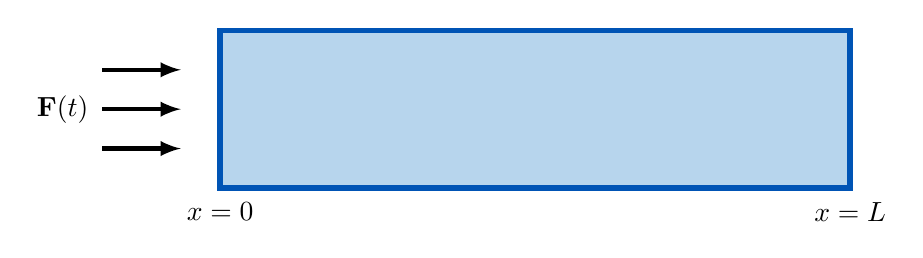
\begin{tikzpicture}
		%Grid
%		\draw[line width = 0.05] (0,0) grid (12,12);
	
		% Rectangle
		\draw[line width = 2, blue1, fill = blue2!40] (3,1) rectangle (11,3);
				
		% Force Vectors
		\foreach \x in {0,1,2}
		{
			\draw[shift = {(0,0.5*\x)}, line width = 1.5, ->] (1.5,1.5) -- ++(1,0);
		}
		
		% Nodes
		\node at (1,2) {$\vb{F}(t)$};
		\node at (3,0.7) {$x=0$};
		\node at (11,0.7) {$x=L$};		
	\end{tikzpicture}
	
\end{document}
